
\documentclass[12pt]{article}

% Layout.
\usepackage[top=1.2in, bottom=0.75in, left=1in, right=1in, headheight=1.0in, headsep=0pt]{geometry}

% Fonts.
\usepackage{mathptmx}
\usepackage[scaled=0.86]{helvet}
\renewcommand{\emph}[1]{\textsf{\textbf{#1}}}

% TiKZ.
\usepackage{tikz, pgfplots}
\usetikzlibrary{calc}
\pgfplotsset{my style/.append style={axis x line=middle, axis y line=middle, xlabel={$x$}, ylabel={$y$}}}
\pgfplotsset{compat=1.16}

% Misc packages.
\usepackage{amsmath,amssymb,latexsym,bm,array,multicol,enumitem}
\usepackage{graphicx}
\usepackage{xcolor}

% Commands to set various header/footer components.
\makeatletter
\def\doctitle#1{\gdef\@doctitle{#1}}
\doctitle{Use {\tt\textbackslash doctitle\{MY LABEL\}}.}
\def\docdate#1{\gdef\@docdate{#1}}
\docdate{Use {\tt\textbackslash docdate\{MY DATE\}}.}
\def\doccourse#1{\gdef\@doccourse{#1}}
\let\@doccourse\@empty
\def\docscoring#1{\gdef\@docscoring{#1}}
\let\@docscoring\@empty
\def\docversion#1{\gdef\@docversion{#1}}
\let\@docversion\@empty
\makeatother

% Headers and footers layout.
\makeatletter
\usepackage{fancyhdr}
\pagestyle{fancy}
\fancyhf{} % Clears all headers/footers.
\lhead{\emph{\@doctitle\hfill\@docdate} \medskip
\ifnum \value{page} > 1\relax\else\\
\emph{Name: \rule{3.5in}{1pt}\hfill \@docscoring}
\fi}

\rfoot{\emph{\@docversion}}
\lfoot{\emph{\@doccourse}}
\cfoot{\emph{\thepage}}
\renewcommand{\headrulewidth}{0pt}%
\makeatother

% Paragraph spacing
\parindent 0pt
\parskip 6pt plus 1pt

% A problem is a section-like command. Use \problem{5} for a problem worth 5 points.
\newcounter{probcount}
\newcounter{subprobcount}
\setcounter{probcount}{0}

\newcommand{\problem}[1]{%
\par
\addvspace{4pt}%
\setcounter{subprobcount}{0}%
\stepcounter{probcount}%
\makebox[0pt][r]{\emph{\arabic{probcount}.}\hskip1ex}\emph{[#1 points]}\hskip1ex}

\newcommand{\thesubproblem}{\emph{\alph{subprobcount}.}}

% Subproblems are an enumerate-like environment with a consistent
% numbering scheme.  Use \begin{subproblems}\item...\item...\end{subproblems}
\newenvironment{subproblems}{%
\begin{enumerate}[itemindent=8pt,leftmargin=0pt]%
\setcounter{enumi}{\value{subprobcount}}%
\renewcommand{\labelenumi}{\emph{\textsl{\alph{enumi})}} \,}%
}%
{%
\setcounter{subprobcount}{\value{enumi}}%
\end{enumerate}%
}

% Blanks for answers in normal and math mode.
\newcommand{\blank}[1]{\rule{#1}{0.75pt}}
\newcommand{\mblank}[1]{\underline{\hspace{#1}}}
\def\emptybox(#1,#2){\framebox{\parbox[c][#2]{#1}{\rule{0pt}{0pt}}}}

% Misc.
\renewcommand{\d}{\displaystyle}
\newcommand{\ds}{\displaystyle}
\newcommand{\threeopts}{{\small \hspace{-6mm} $\begin{matrix} \text{\textsc{converges}} \\ \text{\textsc{absolutely}} \end{matrix}$ \qquad\qquad $\begin{matrix} \text{\textsc{converges}} \\ \text{\textsc{conditionally}} \end{matrix}$ \qquad\qquad \textsc{diverges}} \bigskip}


\newcommand{\ba}{\mathbf{a}}
\newcommand{\bb}{\mathbf{b}}
\newcommand{\bc}{\mathbf{c}}
\newcommand{\bi}{\mathbf{i}}
\newcommand{\bj}{\mathbf{j}}
\newcommand{\bk}{\mathbf{k}}
\newcommand{\bu}{\mathbf{u}}
\newcommand{\bv}{\mathbf{v}}
\newcommand{\bw}{\mathbf{w}}

\newcommand{\ip}[2]{\mathrm{\left<#1,#2\right>}}
\newcommand{\vv}[2]{\mathrm{\left<#1,#2\right>}}
\newcommand{\vvv}[3]{\mathrm{\left<#1,#2,#3\right>}}



% Solution boxes.
\usepackage[most]{tcolorbox}
\usepgfplotslibrary{fillbetween}
\definecolor{solbg}{RGB}{225,240,252}
\definecolor{solframe}{RGB}{70,130,180}
\newtcolorbox{solution}[1][]{%
  breakable, enhanced,
  colback=solbg, colframe=solframe, boxrule=0.7pt, arc=3pt,
  left=6pt, right=6pt, top=5pt, bottom=5pt,
  before skip=6pt, after skip=6pt,
  fonttitle=\sffamily\bfseries\small, coltitle=white, title={Solution},
  #1}

\doctitle{Math 252: Quiz 2 Solutions}
\docdate{10 September, 2026}
\doccourse{}
\docversion{Solutions}
\docscoring{\fbox{{\LARGE \strut}\hspace{0.8in} / 25}}

\begin{document}
30 minutes maximum.  No aids (book, calculator, etc.) are permitted.
Show all work and use proper notation for full credit.  Answers should
be in reasonably-simplified form.  25 points possible.

\begin{enumerate}
\item Consider the region in the first quadrant bounded by the curves $\ds
  y=\cos\left(x^2\right), y=0, x=0$.
  
\begin{enumerate}
\item (4 points) Sketch the region. {\bf Clearly label any important points}.

\begin{solution}
On $x\ge 0$ the curve $y=\cos\left(x^2\right)$ first meets $y=0$ when $x^2=\frac{\pi}{2}$, so $x=\sqrt{\pi/2}$.
\begin{center}
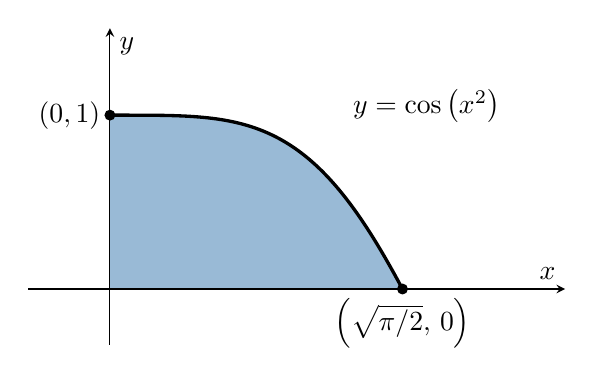
\begin{tikzpicture}
\begin{axis}[my style, axis on top, width=8.4cm, height=5.6cm,
  xmin=-0.35, xmax=1.95, ymin=-0.32, ymax=1.5,
  xtick=\empty, ytick=\empty, clip=false]
\addplot[draw=none, fill=solframe, fill opacity=0.55, domain=0:1.2533141, samples=200] {cos(deg(x^2))} \closedcycle;
\addplot[very thick, domain=0:1.2533141, samples=200] {cos(deg(x^2))};
\node[fill=black, circle, inner sep=1.4pt] at (axis cs:0,1) {};
\node[fill=black, circle, inner sep=1.4pt] at (axis cs:1.2533141,0) {};
\node[left] at (axis cs:0,1) {$(0,1)$};
\node[below] at (axis cs:1.2533141,0) {$\left(\sqrt{\pi/2},\,0\right)$};
\node[anchor=west] at (axis cs:1.0,1.05) {$y=\cos\left(x^2\right)$};
\end{axis}
\end{tikzpicture}
\end{center}
\end{solution}

\item (9 points) Find the volume of the solid
  obtained by rotating the region about the $y$-axis.

\begin{solution}
Rotating about the $y$-axis, a cylindrical shell at $x$ has radius $x$ and height $\cos\left(x^2\right)$:
\[
V=\int_0^{\sqrt{\pi/2}} 2\pi x\cos\left(x^2\right)\,dx .
\]
Substituting $u=x^2$, $du=2x\,dx$, with $u=0$ when $x=0$ and $u=\frac{\pi}{2}$ when $x=\sqrt{\pi/2}$,
\[
V=\pi\int_0^{\pi/2}\cos u\,du=\pi\Bigl[\sin u\Bigr]_0^{\pi/2}=\pi(1-0).
\]
\[
\boxed{\ V=\pi\ }
\]
\end{solution}
  \end{enumerate}

  \newpage

\item (6 points) Set up, but {\bf do not evaluate} an integral that computes
  the arc length of the curve $y=x^4$ from the point $(-1,1)$ to the point $(1,1)$.

\begin{solution}
$y'=4x^3$, and the two points correspond to $x=-1$ and $x=1$, so
\[
L=\int_{-1}^{1}\sqrt{1+\left(4x^3\right)^2}\,dx .
\]
\[
\boxed{\ L=\int_{-1}^{1}\sqrt{1+16x^6}\,dx\ }
\]
\end{solution}

\item (6 points) Set up, but {\bf do not evaluate} an integral that computes
  the surface area of the solid obtained by rotating the curve
  $y=\cos(x)$ over the interval $\left[ -\frac{\pi}{2},\frac{\pi}{2}
  \right]$ about the $x$-axis.

\begin{solution}
$y'=-\sin(x)$, and the radius of revolution is $y=\cos(x)$, which is nonnegative on $\left[-\frac{\pi}{2},\frac{\pi}{2}\right]$.
\[
S=\int_{-\pi/2}^{\pi/2} 2\pi\cos(x)\sqrt{1+\left(-\sin(x)\right)^2}\,dx .
\]
\[
\boxed{\ S=\int_{-\pi/2}^{\pi/2} 2\pi\cos(x)\sqrt{1+\sin^2(x)}\,dx\ }
\]
\end{solution}

  BONUS (2 points) Find the arc length of the curve $\ds y = \sqrt{9 -
    x^2}$ from the point $(-3,0)$ to $(0,3)$. Justify your answer.

\begin{solution}
Squaring gives $x^2+y^2=9$ with $y\ge 0$, so the curve is the upper half of the circle of radius $3$ centered at the origin.  The points $(-3,0)$ and $(0,3)$ are a quarter turn apart on that circle, so the arc is one quarter of the full circumference $2\pi(3)=6\pi$.
\[
\boxed{\ L=\frac{3\pi}{2}\ }
\]
\end{solution}


\end{enumerate}


\end{document}

%-------------------------------------------------------------------------------------------------------------------------------------------------------------------------------------------------------------------

%%% Local Variables:
%%% mode: latex
%%% TeX-master: t
%%% End:
